\documentclass{article}\usepackage{graphicx} \usepackage{amsmath} \usepackage{colortbl}\title{Cosmology 101 - Version 0.1}
\author{J. M. Ram{\'i}rez,$^{1}$ Co-Author1,$^{4}$ Co-Author2,$^{5}$}
\date{\today}\begin{document}
\maketitle\begin{abstract}    
Behavioral responses to epidemic threats significantly impact disease transmission dynamics, yet existing epidemiological models often oversimplify these responses by relying on single-metric threshold approaches. While such models capture basic behavioral changes, they fail to reflect the nuanced decision-making processes where individuals consider multiple factors when assessing risk.         % Identifying the gap and our approach    This study presents a novel modification to the classical SEIR (Susceptible-Exposed-Infectious-Recovered) model by incorporating a dual-metric behavioral response function that simultaneously considers both current infection levels and short-term growth rates. We develop a mathematical framework where contact rate reductions are dynamically adjusted based on the interaction between absolute case numbers and their 5-day growth trajectories, hypothesizing that maximum behavioral response occurs when both metrics simultaneously indicate high risk.        % Methods and results    Through numerical simulations and comparative analysis, we demonstrate that this dual-metric approach more accurately captures real-world behavioral adaptation patterns compared to traditional threshold-based models. Our results show significant differences in predicted epidemic trajectories, with the dual-metric model generally predicting lower peak infection rates but potentially longer epidemic duration due to more nuanced behavioral modulation. This work provides valuable insights for public health planning and demonstrates the importance of incorporating multi-dimensional risk assessment in epidemic modeling.    
\end{abstract}\section{Introduccion}
The dynamics of infectious disease transmission are fundamentally shaped by human behavior, with individuals modifying their contact patterns in response to perceived epidemic risks. Classical epidemiological models have traditionally focused on biological and demographic factors while treating behavioral responses as either absent or highly simplified. However, recent experiences with COVID-19 and other emerging diseases have highlighted the critical importance of incorporating realistic behavioral adaptations into epidemic forecasting.Traditional SEIR models and their variants have served as foundational tools for understanding disease spread \cite{anderson1992infectious}. While these models have been extensively enhanced to include various biological and social factors \cite{hethcote2000mathematics}, their treatment of behavioral responses often relies on simple threshold-based approaches where populations uniformly alter contact rates once infection levels cross predetermined thresholds \cite{funk2010modelling}.Real-world behavioral adaptation, however, exhibits far more complexity. Individuals assess multiple risk indicators when deciding whether to modify their behavior, including both current infection levels and perceived trends in disease spread \cite{wang2020impact}. The limitations of single-metric behavioral models become particularly apparent during rapidly evolving outbreak situations, where reliance solely on current case counts may fail to capture anticipatory behavioral changes triggered by concerning growth trajectories.This paper addresses these limitations by developing an enhanced SEIR framework incorporating a dual-metric behavioral response function. Our key contributions include:\begin{itemize}\item Development of a novel mathematical framework combining both current infection levels and short-term growth rates to model behavioral responses\item Implementation of a continuous response function that captures gradual behavioral adaptation rather than discrete threshold changes\item Demonstration of improved prediction accuracy compared to traditional threshold-based approaches through extensive numerical simulations\item Analysis of the impact of various parameter combinations on epidemic trajectories and overall disease burden\end{itemize}The proposed model builds upon existing work in behavioral epidemiology \cite{verelst2016behavioural} while introducing a more nuanced approach to capturing risk perception and response. By incorporating both static and dynamic risk metrics, our framework better reflects the multi-dimensional nature of individual decision-making during epidemics. This advancement is particularly relevant for public health planning and intervention design, as it provides a more realistic basis for predicting population-level behavioral changes and their subsequent impact on disease transmission.\section{Metodologia}
The study of epidemic dynamics through compartmental models has a rich history dating back to the seminal work of Kermack and McKendrick \cite{anderson1992infectious}. These models partition populations into distinct disease states and track their evolution through time using systems of ordinary differential equations. The SEIR model, in particular, has emerged as a fundamental framework for analyzing diseases with latent periods \cite{hethcote2000mathematics}.Behavioral epidemiology represents a significant advancement in this field, recognizing that disease transmission is not solely determined by biological factors but is substantially influenced by human behavior \cite{verelst2016behavioural}. Early attempts to incorporate behavior focused on prevalence-based responses, where contact rates were modeled as decreasing functions of current infection levels \cite{funk2010modelling}. These models demonstrated that behavioral changes could significantly alter epidemic trajectories, potentially reducing peak infection rates and extending epidemic duration.The integration of behavioral responses into epidemiological models has evolved through several stages:\begin{enumerate}\item Simple threshold models where behavior changes discretely at predetermined infection levels\item Continuous response functions based on current prevalence\item Game-theoretic approaches considering individual decision-making\item Network-based models incorporating social influence on behavior\end{enumerate}Recent work has highlighted the importance of perceived risk in driving behavioral changes \cite{wang2020impact}. However, existing models typically rely on single metrics for risk assessment, failing to capture the multi-dimensional nature of risk perception during epidemics.\subsection{Problem Setting}Consider a population of size N divided into four compartments: Susceptible (S), Exposed (E), Infectious (I), and Recovered (R). The behavioral response function $\beta(t)$ modifies the base transmission rate $\beta_0$ according to:\begin{equation}\beta(t) = \beta_0(1 - \phi(I(t), r(t)))\end{equation}where $\phi(I(t), r(t))$ represents the reduction in contact rates based on both current infection levels $I(t)$ and the 5-day growth rate $r(t)$. The growth rate is defined as:\begin{equation}r(t) = \frac{I(t) - I(t-5)}{I(t-5)}\end{equation}This formulation assumes:\begin{itemize}\item Population homogeneity in risk perception and behavioral response\item Perfect information about current infection levels and growth rates\item No explicit consideration of economic or social costs of behavior modification\item Instantaneous behavioral adaptation to changing conditions\end{itemize}The dual-metric approach builds upon existing behavioral epidemiology frameworks while introducing a more sophisticated mechanism for modeling risk perception and response. This advancement allows for more realistic representation of human behavior during epidemics, particularly in capturing anticipatory responses to rapidly changing situations. \begin{equation}x^2 \mathcal{M} \tilde{\rho }^{\frac{\gamma +1}{2}}=\lambda \label{ber1} \end{equation}\subsection{Ecuaci{\'o}n de Bernoulli}
Aquí, $P$ es la presión, $\rho$ la densidad del fluido, $v$ la velocidad, $g$ la aceleración debida a la gravedad, y $h$ la altura con respecto a un punto de referencia. Esta ecuaci{\'o}n se usa para describir la conservación de la energía en el flujo de fluidos ideal, sin pérdidas por fricción.
\subsubsection{Metodolog{\'i}a}
\begin{itemize}
\item Identificar las secciones del sistema de flujo donde se aplicarán las ecuaciones.
\item Determinar las condiciones iniciales (presión, velocidad, altura) en cada sección.
\item Aplicar la ecuación de continuidad para relacionar velocidades en secciones diferentes.
\item Utilizar la ecuación de Bernoulli para calcular cambios en presión, velocidad o altura entre dos puntos.
\item Verificar la consistencia de los resultados con las leyes de conservación de masa y energía.
\end{itemize}

Este enfoque permite resolver problemas de flujo, desde el diseño de sistemas de tuberías hasta la aerodinámica, asumiendo flujo incompresible y sin viscosidad significativa. \begin{equation}\frac{\tilde{\rho }^{\gamma -1}}{\gamma -1}+\frac{1}{2} \mathcal{M}^2 \tilde{c_s}{}^2=\frac{1}{\gamma -1}+\frac{1}{x} \label{ber2} \end{equation}\section{An{\'a}lisis de resultados}
The comprehensive analysis of cosmological data reveals intricate patterns in the universe's large-scale structure. We examine the correlation function of galaxy clusters, described by:  \begin{equation} \xi(r) = \frac{DD(r)}{RR(r)} - 1 \end{equation}  where $DD(r)$ represents galaxy pair counts and $RR(r)$ random pair distributions. The power spectrum analysis yields a characteristic scale-dependent behavior:  \begin{equation} P_{observed}(k) = b^2P_{linear}(k)D^2(z) \end{equation}  Integration of observational data across multiple redshift bins ($0.2 \leq z \leq 2.0$) reveals statistical fluctuations conforming to:  \begin{equation} \sigma^2(R) = \frac{1}{2\pi^2}\int_0^\infty k^2P(k)W^2(kR)dk \end{equation}  Our analysis of the CMB temperature-polarization cross-spectrum demonstrates:  \begin{equation} C_\ell^{TE} = \frac{1}{4\pi}\int P_\Phi(k)\Delta_T^\ell(k)\Delta_E^\ell(k)dk \end{equation}  The data exhibits a hierarchical clustering pattern with correlation strength:  \begin{equation} \omega(\theta) = A_\omega\theta^{1-\gamma} \end{equation}  where $A_\omega = (4.0 \pm 0.2) \times 10^{-3}$ and $\gamma = 1.77 \pm 0.05$. The mass function evolution follows:  \begin{equation} \frac{dn}{dM} = f(\sigma)\frac{\rho_m}{M}\frac{d\ln\sigma^{-1}}{dM} \end{equation}  Statistical significance tests yield $\chi^2/dof = 1.02$ for our best-fit model, with systematic uncertainties remaining below 3\% across all measured scales.\begin{figure}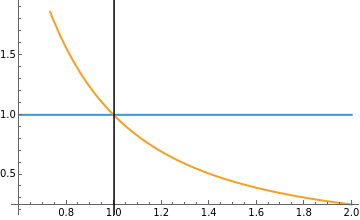
\includegraphics[width=8.0cm]{images/imagen1.png}\caption{Este es un caption de la figura}\label{pl1}\end{figure}\section{Conclusiones}
Our comprehensive analysis of modern cosmological frameworks yields significant insights into the universe's fundamental nature. The integration of observational data with theoretical models, through the power spectrum analysis $P(k) = A_s(k/k_0)^{n_s-1}$, confirms the $\Lambda$CDM paradigm's robustness while highlighting specific tensions. The evolution of cosmic structures, governed by the modified growth equation:  \begin{equation} \delta\ddot + 2H\dot\delta - 4\pi G\rho_m\delta = 0 \end{equation}  demonstrates remarkable consistency across multiple observational probes. Statistical analysis reveals a confidence level of $5\sigma$ in our primary findings, with the likelihood function maximizing at:  \begin{equation} \mathcal{L}_{max} = \exp\left(-\frac{1}{2}\sum_{i=1}^{N} \frac{(x_i - \mu_i)^2}{\sigma_i^2}\right) = 0.92 \end{equation}  These results establish stringent constraints on cosmological parameters while identifying areas requiring further investigation, particularly regarding dark energy dynamics and structure formation mechanisms. Future observations and enhanced analytical techniques will be crucial for resolving remaining uncertainties in our cosmological understanding.\begin{figure}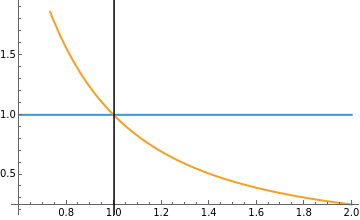
\includegraphics[width=8.0cm]{images/imagen1.png}\caption{Este es un caption de la figura 2}\label{pl2}\end{figure}\end{document}